\documentclass[usenames,dvipsnames, 9pt]{beamer}
\usepackage{amsmath,amsfonts,amssymb}
\usepackage{mathtools}
\usepackage{etex} %for Windows
\usepackage[utf8]{inputenc}
\usepackage[english, russian]{babel} 

%\usepackage{microtype}			% Better interword spacing and additional kerning.
\usepackage{ellipsis}			% Adjusted space with \dots between two words.
\usepackage{graphicx}
\usepackage{pstricks}

\usepackage{xcolor}


\usepackage{changepage}

\usepackage{algorithm}
\usepackage{algpseudocode}
%\usepackage[]{algorithm2e}
%\usepackage{algorithmic}

%\usepackage{tcolorbox}






\usepackage{tikz}
\usetikzlibrary{tikzmark,calc}
\usetikzlibrary{positioning, backgrounds}
\usetikzlibrary{arrows, chains, matrix, scopes, patterns, shapes, fit}
\usetikzlibrary{mindmap,trees,shadows}
\usetikzlibrary{decorations.pathreplacing}

\usepackage{pgfplots}

\pgfmathdeclarefunction{gauss}{2}{%
	\pgfmathparse{1/(#2*sqrt(2*pi))*exp(-((x-#1)^2)/(2*#2^2))}%
}


\tikzset{
	invisible/.style={opacity=0},
	visible on/.style={alt={#1{}{invisible}}},
	alt/.code args={<#1>#2#3}{%
		\alt<#1>{\pgfkeysalso{#2}}{\pgfkeysalso{#3}} % \pgfkeysalso doesn't change the path
	},
}

\newcommand\strikeout[2][]{%
	\begin{tabular}[b]{@{}c@{}} 
		\makebox(0,0)[cb]{{#1}} \\[-0.2\normalbaselineskip]
		\rlap{\color{Orange}\rule[0.5ex]{\widthof{#2}}{1.5pt}}#2
\end{tabular}}

\newcommand\Fontvi{\fontsize{11}{13.2}\selectfont}

\usepackage{listings} % for C++ code

\usepackage{braket}
%\usepackage[braket, qm]{qcircuit}



\usepackage[T1]{fontenc}
%\usepackage[sfdefault,scaled=.85]{FiraSans}
%\usepackage{newtxsf}
%\usepackage[nomap]{FiraMono}





\usefonttheme[onlymath]{serif}
\renewcommand\sfdefault{cmbr}

\renewcommand{\bfdefault}{sb}




\definecolor{CharCoalDark}{RGB}{13, 16, 19}
\definecolor{Orange}{RGB}{255, 165,0}
\definecolor{DarkOrange}{RGB}{255, 165,0}
\definecolor{LightSalmon}{RGB}{255, 160, 122}
\definecolor{LeafGreen}{RGB}{34, 139,  34}
\definecolor{Coral}{RGB}{255, 127, 80}
\definecolor{DarkTurquoise}{RGB}{0, 206, 209}

%\newtheorem{defRus}{Определение}
%\newtheorem{thmRus}{Теорема}
%s\newtheorem{corRus}{Следствие}


\setbeamercolor{background canvas}{bg=CharCoalDark}

\setbeamerfont{title}{series=\bfseries}
\setbeamercolor{title}{fg=Orange}
\setbeamercolor{section in toc}{fg=white}
\setbeamercolor{frametitle}{fg=Orange}
\setbeamercolor{normal text}{fg=white}
%\setbeamercolor{normal text}{fontsize=12pt}
\setbeamercolor{itemize item}{fg=Orange}
\setbeamercolor{itemize item item}{fg=Orange}
\setbeamercolor{enumerate item}{fg=Orange}
\setbeamercolor{itemize subitem}{fg=Orange}
\setbeamercolor{enumerate subitem}{fg=Orange}
\setbeamercolor{block title}{bg=DarkOrange,fg=white}
\setbeamerfont{block title}{series=\bfseries}

\setbeamertemplate{itemize item}[circle]
%\setbeamertemplate{itemize subitem}[$\checkmark$]
%\setbeamertemplate{itemize subitem}{\color{Orange}\Large${\checkmark}$}
\setbeamertemplate{itemize subitem}{\color{Orange}\Large $\blacksquare$}

% footnote without a marker
\newcommand\blfootnote[1]{%
	\begingroup
	\renewcommand\footnoterule{}
	\renewcommand\thefootnote{}\footnote{#1}%
	\addtocounter{footnote}{-1}%
	\endgroup
}

\newcommand*{\Scale}[2][4]{\scalebox{#1}{\ensuremath{#2}}}%


\AtBeginSection[]
{
	\begin{frame}<beamer>
		\frametitle{Outline}
		\tableofcontents[currentsection]
	\end{frame}
}

\newcommand\myineq{\stackrel{\mathclap{\normalfont\mbox{?}}}{\approx}}



%\institute{ENS Lyon}
\author{Елена Киршанова \\ [10pt]
	%based on joint works with G.Herold, T.Laarhoven
}
\titlegraphic{
	%\includegraphics[width=2.5cm]{erc_logo_gray}\hspace*{2.5cm}~%
	%\hspace*{1.0cm}
\includegraphics[width=4.0cm]{GC_BFU_logo_full_cyr_bw}
}
\title{\Large{Современная криптография на решётках}}

\date{ Курс ``Криптография на решётках'' \\  }


\setbeamertemplate{navigation symbols}{} %removes navigation

% proper highlightling of a code-snippet
\lstset{language=C++,
	keywordstyle=\color{magenta},
	stringstyle=\color{Goldenrod},
	commentstyle=\color{gray},
	breaklines=false,
	%morecomment=[l][\color{magenta}]{\#}
}

\setlength{\parskip}{8pt}

% ==================================================================
% Definitions for this paper
% ==================================================================
\mathchardef\hyphen="2D

\usepackage{multirow}
\usepackage{multicol} % For multiple coloumn environments
%\usepackage{stmaryrd} % For set brackets
% \setlength{\columnsep}{15pt} % Defining the coloumn seperation
% \setlength{\columnseprule}{1pt} % Place a line between coloumns
% \newcommand{\tab}{\hspace*{2em}}

%subscripts

\newcommand*\SmallTextScript[2]{{\mathchoice{\displaystyle #2}
		{\textstyle #2}%dito
		{\scalebox{#1}{\ensuremath{\scriptstyle #2}}}%
		{\scalebox{#1}{\ensuremath{\scriptscriptstyle #2}}}%
}}


% ADVERSARIES AND SUCH
\newcommand*{\poly}{\ensuremath{\mathrm{poly}}}
\newcommand*{\eps}{\ensuremath{\varepsilon}}
\newcommand*{\alg}{\ensuremath{\mathcal{A}}}

% GROUPS/DISTRIBUTIONS/SETS/LISTS
\newcommand{\N}{{{\mathbb N}}}
\newcommand{\Z}{{{\mathbb Z}}}
\newcommand*{\IZ}{\ensuremath{\mathbb{Z}}}
\newcommand*{\IN}{\ensuremath{\mathbb{N}}}
\newcommand*{\IQ}{\ensuremath{\mathbb{Q}}}
\newcommand{\R}{{{\mathbb R}}}
\newcommand*{\IR}{{{\mathbb R}}}
\newcommand{\Zp}{\ints_p} % Integers modulo p
\newcommand{\Zq}{\ints_q} % Integers modulo q
\newcommand{\Zn}{\ints_N} % Integers modulo N
\newcommand{\F}{\ensuremath{\mathbb{F}}}
\newcommand{\CC}{\ensuremath{\mathbb{C}}}

\newcommand{\GF}{\ensuremath{\mathbb{F}_2}}
\newcommand{\GFn}{\ensuremath{\mathbb{F}^n_2}}

%%% ALGORITHMS/PROCEDURES %%%
\newcommand{\Dec}{\textsf{Dec}}
\newcommand{\Enc}{\textsf{Enc}}
\newcommand{\KeyGen}{\textsf{KeyGen}}
\newcommand{\Gen}{\textsf{Gen}}
\newcommand{\sk}{\textsf{sk}}
\newcommand{\pk}{\textsf{pk}}
\newcommand{\vk}{\textsf{vk}}
\newcommand{\mesS}{\ensuremath{\mathcal{M}}}
\newcommand{\keyS}{\ensuremath{\mathcal{K}}}
\newcommand{\cipS}{\ensuremath{\mathcal{C}}}
\newcommand{\tagS}{\ensuremath{\mathcal{T}}}
\newcommand{\mactag}{\textsf{tag}}
\newcommand{\Hash}{\ensuremath{\mathcal{H}}}
\newcommand{\EID}{\ensuremath{\mathtt{EphID}}}


\newcommand{\adv}{\ensuremath{\mathcal{A}}}

\newcommand{\LWE}{\mathsf{LWE}}
\newcommand{\DCP}{\mathsf{DCP}}
\newcommand{\EDCP}{\mathsf{EDCP}}
\newcommand{\UEDCP}{\mathsf{U \text{-} EDCP}}
\newcommand{\GEDCP}{\mathsf{G \text{-} EDCP}}



%% Landau and proba
\newcommand{\bigO}{\mathcal{O}}
\newcommand*{\OLandau}{\bigO}
\newcommand*{\WLandau}{\Omega}
\newcommand*{\xOLandau}{\widetilde{\OLandau}}
\newcommand*{\xWLandau}{\widetilde{\WLandau}}
\newcommand*{\TLandau}{\Theta}
\newcommand*{\xTLandau}{\widetilde{\TLandau}}
\newcommand{\smallo}{o} %technically, an omicron
\newcommand{\wLandau}{\omega}
\newcommand{\negl}{\mathrm{negl}}
\newcommand*\PROB\Pr 
\DeclareMathOperator*{\EXPECT}{\mathbb{E}}
\DeclareMathOperator*{\VARIANCE}{\mathbb{V}}
\DeclareMathOperator*{\LOGBIAS}{\mathbb{LB}}

\newcommand{\supp}{\ensuremath{\mathsf{sup}}}
\newcommand{\Distr}{\ensuremath{\mathcal{D}}}

% Lattices

% \newcommand{\coset}{\Lambda} % Lambda Lattice
% \newcommand{\cosetPerp}{\Lambda^{\bot}} % Lambda_Perp Lattice
% \newcommand{\gadget}{\textbf{G}} %Gaget matrix
% \newcommand{\mes}{\textbf{m}} %message vector
% \newcommand{\AMat}{\textbf{A}} %A matrices
% \newcommand{\BMat}{\textbf{B}} %B matrices
% \newcommand{\RMat}{\textbf{R}} %R matrices
% \newcommand{\HMat}{\textbf{H}} %H matrices
% \newcommand{\XMat}{\textbf{X}} %H matrices
% \newcommand{\mbar}{\bar{m}} %mBar dimension
% % \newcommand{\gauss}{\mathcal{D}} % gaussian distribution
% \newcommand{\Id}{\textbf{I}} % Identity matrix
% \newcommand{\er}{\textbf{e}} % gaussian distr. vectors
% % \newcommand{\cipher}{\textit{c}} % ciphertext
% \newcommand{\Olwe}{\mathcal{O}_{\textsf{LWE}}} %LWE oracle
% \newcommand{\OSample}{\mathcal{O}_{Sample}} %LWE oracle
% \newcommand{\SigmaB}{\boldsymbol{\Sigma}} %semi-deifinite matrix Sigma%
% % \newcommand{\mods}{\text{ mod}}


%Vectors and Matrices

\newcommand{\AMat}{\mathbf{A}} %A matrices
\newcommand{\BMat}{\mathbf{B}} %B matrices
\newcommand{\DMat}{\mathbf{D}} %Diagonal


\newcommand{\HMat}{\ensuremath{\mathbf{H}}}
\newcommand{\QMat}{\ensuremath{\mathbf{Q}}}
\newcommand{\Id}{\ensuremath{\mathbf{I}}}
\newcommand{\ZeroM}{\textbf{0}} % Zero matrix

\newcommand{\avec}{\ensuremath{\mathbf{a}}}
\newcommand{\bvec}{\ensuremath{\mathbf{b}}}
\newcommand{\cvec}{\ensuremath{\mathbf{c}}}
\newcommand{\evec}{\ensuremath{\mathbf{e}}}
\newcommand{\rvec}{\ensuremath{\mathbf{r}}}
\newcommand{\svec}{\ensuremath{\mathbf{s}}}
\newcommand{\tvec}{\ensuremath{\mathbf{t}}}
\newcommand{\vvec}{\ensuremath{\mathbf{v}}}
\newcommand{\zvec}{\ensuremath{\mathbf{z}}}
\newcommand{\xvec}{\ensuremath{\mathbf{x}}}
\newcommand{\yvec}{\ensuremath{\mathbf{y}}}
\newcommand{\uvec}{\ensuremath{\mathbf{u}}}
\newcommand{\zerovec}{\ensuremath{\mathbf{0}}}

\newcommand{\nth}{^{\mathrm{th}}}
\newcommand{\nd}{^{\mathrm{nd}}}

\newcommand{\RepMMT}{\ensuremath{\mathcal{R}_{\protect\SmallTextScript{0.70}{\texttt{MMT}}}}}
\newcommand{\RepBJMM}{\ensuremath{\mathcal{R}_{\protect\SmallTextScript{0.70}{\texttt{BJMM}}}}}
\newcommand{\XOR}{\ensuremath{\mathtt{3XOR}}}


% % % % % \newcommand{\mb}[1]{\mathbf{#1}} % does not compile otherwise
%%% Removed by Gotti; this is just asking to screw up with packages that (properly) define \mb (mathbold)

% \newcommand{\bL}{\|\bvec_1\|} % b1 length that appears way too often
% \newcommand{\dL}{\|\dvec_1\|} % b1 length that appears way too oftend

%Norms and Scalar products

\newcommand*\abs[1]{\left\lvert#1\right\rvert}
\newcommand*\norm[1]{\left\lVert#1\right\rVert}
\newcommand*\normalabs[1]{\lvert#1\rvert} 
\newcommand*\normalnorm[1]{\lVert#1\rVert}
\newcommand*\bignorm[1]{\bigl\lVert#1\bigr\rVert}
\newcommand*\bigabs[1]{\bigl\lvert#1\bigr\rvert}
\newcommand*\Bigabs[1]{\Bigl\lvert#1\Bigr\rvert}
\newcommand*{\ScProd}[2]{\ensuremath{\langle#1\mathbin{,}#2\rangle}} %Scalar Product
% \newcommand*{\ScProd}[2]{\ensuremath{\langle#1 \:{,}\:#2\rangle}} %Scalar Product
\newcommand*{\bigScProd}[2]{\ensuremath{\bigl\langle#1\mathbin{,}#2\bigr\rangle}} %Scalar Product
\newcommand*{\BigScProd}[2]{\ensuremath{\Bigl\langle#1\mathbin{,}#2\Bigr\rangle}} %Scalar Product
\newcommand{\dist}{\ensuremath{\text{dist}}}


%Some other math operators

\DeclareMathOperator{\Span}{Span} %span of vectors
\DeclareMathOperator{\vol}{\mathrm{vol}} %volume
\DeclareMathOperator{\LW}{LambertW} %Lambert W function
\DeclareMathOperator{\SD}{SD}
\DeclareMathOperator{\gradient}{grad}
\DeclareMathOperator{\TRACE}{Tr}
\newcommand*{\dDR}{\mathrm{d}} %de-Rham-Differential (the d in dx, dy, dz and so on)


%Lists
\renewcommand{\L}{\ensuremath{\mathcal{L}}}

\renewcommand{\P}{\ensuremath{\mathcal{P}}}

\newcommand*{\Lout}{\ensuremath{\L_{\mkern-0.5mu\protect\SmallTextScript{0.85}{\textup{out}}}}}
\newcommand*{\Sout}{\ensuremath{S_{\mkern-0.5mu\protect\SmallTextScript{0.85}{\textup{out}}}}}
\newcommand{\wt}{\ensuremath{\mathit{wt}}}


\newcommand*{\softO}{\widetilde{\bigO}}

\newcommand{\const}{\mathsf{c}} 


\newcommand{\transpose}{\mkern0.7mu^{\mathsf{ t}}}

%proper overline reduced by 1.5mu
\newcommand{\overbar}[1]{\mkern 1.5mu\overline{\mkern-1.5mu#1\mkern-1.5mu}\mkern 1.5mu}

\DeclareMathOperator{\erf}{erf} %error function
\DeclareMathOperator{\erfc}{erfc} %complementary error function
\newcommand{\Er}{\ensuremath{\mathrm{Er}}} %complementary error function


% LATTICES

\newcommand{\Lat}{\ensuremath{\mathcal{L}}}
\newcommand*{\Sphere}[1]{\ensuremath{\mathsf{S}^{#1}}}
%\DeclareMathOperator{\Conf}{Conf}
\newcommand{\Conf}{\mathcal{C}}

%Thick line for table
\setlength{\doublerulesep}{0pt}
\newcommand{\thickline}{\hline\hline\hline}


%circled text
\newcommand*\circled[1]{\tikz[baseline=(char.base)]{
    \node[shape=circle,draw,inner sep=0.3 pt] (char) {\scriptsize #1};}}


%Fix Algorithmicx package
\def\NoNumber#1{{\def\alglinenumber##1{}\State #1}\addtocounter{ALG@line}{-1}}

%For comments
\newcommand{\GColor}{ForestGreen}  %Damiens' color
\newcommand{\EColor}{MidnightBlue} %Elena's color

\newcommand*{\E}[1]{{\color{\EColor} #1} } 
\newcommand*{\G}[1]{{\color{\GColor} #1} } 

%Proper limit with the subscript underneath
% \newcommand{\Lim}[1]{\raisebox{0.5ex}{\scalebox{0.8}{$\displaystyle \lim_{#1}\;$}}}


%TIKZ dense dotted pattern

\pgfdeclarepatternformonly{my dots}{\pgfqpoint{-1pt}{-1pt}}{\pgfqpoint{2.0pt}{2.0pt}}{\pgfqpoint{2pt}{2pt}}%
{
	\pgfpathcircle{\pgfqpoint{0pt}{0pt}}{.35pt}
	\pgfpathcircle{\pgfqpoint{1pt}{1pt}}{.35pt}
	\pgfusepath{fill}
}


\tikzset{
	master/.style={
		execute at end picture={
			\coordinate (lower right) at (current bounding box.south east);
			\coordinate (upper left) at (current bounding box.north west);
		}
	},
	slave/.style={
		execute at end picture={
			\pgfresetboundingbox
			\path  (lower right)rectangle (upper left) ;
		}
	}
} %all defs
\begin{document}
	
\begin{frame}
	\titlepage
\end{frame}

%\begin{frame}{Outline}
%	\tableofcontents
%\end{frame}



%\section{Definitions}

\begin{frame}{Трудные задачи на решётках: SIS}
	\begin{tikzpicture}[scale=0.9]
	\draw[fill=CharCoalDark, draw=white, opacity=0.5] (-6.0,4.0) rectangle (-4.5,7.0) node[color=white, opacity=1,align=center, pos=0.5] {
			\Huge  $A$
		}; 
	\draw[stealth-stealth] (-6.2,4.0) -- (-6.2,7.0) node[midway, xshift=-6pt] {\LARGE $m$};
	\draw[stealth-stealth] (-6.0,3.9) -- (-4.5,3.9) node[midway, yshift=-6pt] {\LARGE $n$};
	
	
	\draw[-latex, very thick] (-4.3, 5.5) -- (-2.8, 5.5) node[above, xshift=-20pt]{\large найти $\xvec$: };
	\draw[|-|, draw=Orange, very thick] (-3.0, 6.8) -- (-0.2, 6.8) node[midway, above]{\LARGE $\xvec$};
	\draw[fill=CharCoalDark, draw=white, opacity=0.5] (0.0,4.0) rectangle (1.5,7.0) node[color=white, opacity=1,align=center, pos=0.5] {
			\Huge  $A$
		}; 
	\draw(3.0, 5.5)node{\LARGE $= \zerovec \bmod~q$};
	\draw(-0.0, 3.2)node{\LARGE т.ч. $0 < \norm{\xvec} \leq B$};
	
	%
	%\draw(-1.8, 5.5)node{\Huge $+$};
	%
	%\draw[|-|, draw=Orange, very thick] (-1.3, 4.0) -- (-1.3, 7.0) node[above]{\LARGE $\evec$};
	%
	%\draw(-0.5, 5.5)node{\Large $\bmod~q$};
	
	%
	%\draw[|-|, draw=Orange, very thick] (2.0, 5.5) -- (2.0, 7.0) node[above]{\LARGE $\svec$};
	%\draw(2.5, 5.5)node{\Large or};
	%\draw[|-|, draw=Orange, very thick] (3.0, 4.0) -- (3.0, 7.0) node[above]{\LARGE $\evec$};
	\end{tikzpicture}
	\vspace{-10pt} 
	\pause
	\Large 	
	\begin{itemize}
		\setlength\itemsep{5pt}

		\item $A$ задаёт решётку ранга $m$
		\[
		\Lat_q^\perp(A) = \{ \xvec \in \Z^m \; : \; \xvec\transpose A = 0 \bmod q \}
		\]
		\item SIS -- $\gamma$-SVP для $\gamma = \frac{q^{n/m}}{B}$. %Analogously to LWE,
		\[
			T(\text{SIS}) = \exp\left(\const  \frac{\lg q}{\lg^2 B} \lg\Big( \frac{n \lg q}{\lg^2 B} \Big)  \cdot n\right)
		\] 
		\item Криптографические хэш-функции, цифровые подписи
	\end{itemize}
	
	
\end{frame}

\begin{frame}{Трудные задачи на решётках: LWE}
		\begin{tikzpicture}
		\draw[fill=CharCoalDark, draw=white, opacity=0.5] (-6.0,4.0) rectangle (-4.5,7.0) node[color=white, opacity=1,align=center, pos=0.5] {
			\Huge  $A$
		}; 
		\draw[stealth-stealth] (-6.2,4.0) -- (-6.2,7.0) node[midway, xshift=-6pt] {\LARGE $m$};
		\draw[stealth-stealth] (-6.0,3.9) -- (-4.5,3.9) node[midway, yshift=-6pt] {\LARGE $n$};
		
		\draw(-4.3, 5.5)node{\Huge ,};
		
		\draw[fill=CharCoalDark, draw=white, opacity=0.5] (-4.0,4.0) rectangle (-2.5,7.0) node[color=white, opacity=1,align=center, pos=0.5] {
			\Huge  $A$
		}; 
		
		\draw[|-|, draw=Orange, very thick] (-2.3, 5.5) -- (-2.3, 7.0) node[above]{\LARGE $\svec$};
		
		\draw(-1.8, 5.5)node{\Huge $+$};
		
		\draw[|-|, draw=Orange, very thick] (-1.3, 4.0) -- (-1.3, 7.0) node[above]{\LARGE $\evec$};
		
		\draw(-0.5, 5.5)node{\Large $\bmod~q$};
		\draw[-latex, very thick] (0.3, 5.5) -- (1.5, 5.5) node[above, xshift=-20pt]{\large найти};
		
		\draw[|-|, draw=Orange, very thick] (2.0, 5.5) -- (2.0, 7.0) node[above]{\LARGE $\svec$};
		\draw(2.5, 5.5)node{\large или};
		\draw[|-|, draw=Orange, very thick] (3.0, 4.0) -- (3.0, 7.0) node[above]{\LARGE $\evec$};
	\end{tikzpicture}
	
	\vspace{10pt}
	\begin{columns}
		\begin{column}{0.4\textwidth}
			\Huge
			$\begin{array}{c}
				\mkern10mu A \xleftarrow{\$} \Z_q^{m \times n}  \\[3pt]
				\svec  \xleftarrow{\$} \Z_q^n \\ [5pt]
				\mkern7mu \evec  \leftarrow D_{\alpha q}^m \\ 
			\end{array}$
		\end{column}
		\begin{column}{0.5\textwidth}
			\begin{tikzpicture}
				\begin{axis}[every axis plot post/.append style={
						mark=none,domain=-6:6,samples=20,smooth},
					at={(8,8)},
					axis lines*=none,
					axis line style={draw=none},
					tick style={draw=none},
					yticklabels={,,},
					xticklabels={,,},
					height=4.2cm,
					width=7cm
					]
					\addplot[draw=Orange, very thick, dotted] {gauss(0,1.4)};
				\end{axis}
				\draw[stealth-stealth, white] (3,0.2) -- (4,0.2) node[midway, below]{$\alpha q$};
				
				\draw(1, 2.5)node{\LARGE $D_{\alpha q}$};
			\end{tikzpicture}
		\end{column}
	\end{columns}

\end{frame}

\begin{frame}{LWE есть BDD}
\vspace{-8pt}
\begin{tikzpicture}
\draw[fill=CharCoalDark, draw=white, opacity=0.5] (-6.0,4.0) rectangle (-4.5,7.0) node[color=white, opacity=1,align=center, pos=0.5] {
	\Huge  $A$
}; 
\draw[stealth-stealth] (-6.2,4.0) -- (-6.2,7.0) node[midway, xshift=-6pt] {\LARGE $m$};
\draw[stealth-stealth] (-6.0,3.9) -- (-4.5,3.9) node[midway, yshift=-6pt] {\LARGE $n$};

\draw(-4.3, 5.5)node{\Huge ,};

\draw[fill=CharCoalDark, draw=white, opacity=0.5] (-4.0,4.0) rectangle (-2.5,7.0) node[color=white, opacity=1,align=center, pos=0.5] {
	\Huge  $A$
}; 

\draw[|-|, draw=Orange, very thick] (-2.3, 5.5) -- (-2.3, 7.0) node[above]{\LARGE $\svec$};

\draw(-1.8, 5.5)node{\Huge $+$};

\draw[|-|, draw=Orange, very thick] (-1.3, 4.0) -- (-1.3, 7.0) node[above]{\LARGE $\evec$};

\draw(-0.5, 5.5)node{\Large $\bmod~q$};
\draw[-latex, very thick] (0.3, 5.5) -- (1.5, 5.5) node[above, xshift=-20pt]{\Large find};

\draw[|-|, draw=Orange, very thick] (2.0, 5.5) -- (2.0, 7.0) node[above]{\LARGE $\svec$};
\draw(2.5, 5.5)node{\Large or};
\draw[|-|, draw=Orange, very thick] (3.0, 4.0) -- (3.0, 7.0) node[above]{\LARGE $\evec$};
\end{tikzpicture}
\Large
\vspace{-10pt}
\begin{itemize}
	\setlength\itemsep{9pt}
	\item $A$ задает решетку конструкции A
	\[
	\Lat_q(A) = A\Z_q^n + q\Z^m
	\]
	\item  $\dim(\Lat_q(A))=m$  и $\det(\Lat_q(A)) = q^{m-n}$.
	\item $As +e \bmod~q$ -- вектор, на расстоянии  $\Theta(\sqrt{m} \alpha q)$ от $\Lat_q(A)$
	\item $(A,As+e)$  -- {\color{Orange} BDD} задача для $\Lat_q(A)$ с $\gamma = \frac{q^{1-n/m}}{\alpha q} $
	\item PKE, IBE, ABE, NIKZ, гомоморфное шифрование 
	
\end{itemize}

\end{frame}
	
	

\begin{frame}{Алгебраические предположения трудности}
		\Large 
	\begin{itemize}
		\setlength\itemsep{7pt}
		\item Для хранения LWE выборки необходимо $\Omega(n^2 \log q)$ бит
		\item  Умножение матрицы на вектор требует $O(n^2)$ операций в $\Z_q$
	\end{itemize}
	{\color{Orange} $\implies$ `стандартное' LWE довольно медленно }
	
	\vspace{15pt}
	
	\LARGE {\color{Orange}Решение:} 
	\begin{enumerate}
		\setlength\itemsep{5pt}
		\item Алгебраические версии SIS/LWE
		\item NTRU
	\end{enumerate}
\end{frame}

\begin{frame}{Polynomial-LWE, SSTX'09} 
	\LARGE
	Пусть $f \in \Z[x]$ - унитарный неприводимый степени $n$, $q\geq 2, \alpha >0$ \\
	\[
	a = \sum_i a_i x^i \in \Z[x]/f \; \longrightarrow \; (a_0, \ldots, a_{n-1}) \in \Z^n
	\]
	\vspace{-8pt}
	\begin{columns}
		\begin{column}{0.55\textwidth}
			{\color{Orange}Задача поиска $\text{Poly-LWE}_f$:}
			\begin{itemize}
				\item Выбрать ${\color{Orange}s} \xleftarrow{\$} \Z_q[x]/f$
				\item Выбрать $a_i$'s $\xleftarrow{\$} \Z_q[x]/f$
				\item Выбрать {\color{Orange} коэф-ты} ${\color{Orange}e_i}$ из $D_{\alpha q}$
			\end{itemize}
			
			По данным $(a_1, \ldots, a_m)$ и $(a_1 \cdot {\color{Orange}s} + {\color{Orange}e_1}, \ldots a_m \cdot {\color{Orange}s} + {\color{Orange}e_m})$, найти ${\color{Orange}s}$.
		\end{column}
		\pause
		\begin{column}{0.5\textwidth}
			\begin{tikzpicture}[scale=0.70]
				
				\draw[fill=CharCoalDark, draw=white, opacity=0.5] (0.0,6.0) rectangle (3.0,9.0) node[color=white, opacity=1,align=center, pos=0.5] {
					\large $(x^{j-1} \cdot  a_1) [f]$  \\
					= $\text{Rot}_f(a_1)$
				}; 
				\draw[fill=CharCoalDark, draw=white, opacity=0.5] (0.0,3.0) rectangle (3.0,6.0) node[color=white, opacity=1,align=center, pos=0.5] {
					\Large $\text{Rot}_f(a_2)$  
				}; 
				
				\draw[stealth-stealth] (-.2,3.0) -- (-.2,9.0) node[midway, xshift=-16pt] {\large $m\cdot n$};
				\draw[stealth-stealth] (0.0,2.9) -- (3.0,2.9) node[midway, yshift=-6pt] {\large $n$};
				
				\draw[|-|, draw=Orange,  thick] (3.5, 6.0) -- (3.5, 9.0) node[above]{\Large $\svec$};
				\draw(4.2, 6.0)node{\Huge $+$};
				\draw[|-|, draw=Orange,  thick] (4.9, 6.0) -- (4.9, 9.0) node[right, midway]{\Large $\evec_1$};
				\draw[|-|, draw=Orange,  thick] (4.9, 3.0) -- (4.9, 6.0) node[right, midway]{\Large $\evec_2$};
			\end{tikzpicture}
		\end{column}
	\end{columns}
	\pause
	\vspace{-10pt}
	Одна пара $(a_i, a_i s + e_i)$ дает LWE выборку из $n$ эл-тов
	Многочлены могут быть умножены за время $\softO(n)$
\end{frame}

\begin{frame}{Ring-LWE для $f = x^{2^k}+1$, LPR'10} 
	\LARGE
	Пусть $f =x^{n}+1$ - круговой степени $n=2^k$, $q\geq 2, \alpha >0$
	Пусть $\omega_1, \ldots, \omega_n \in \CC$ - корни $f$, $V_f$ - матрица Вандермодна для $\omega_i$'s
	\[
	\sigma:  \sum_i a_i x^i \in \Z[x]/f \; \longrightarrow \;  (a(\omega_0), \ldots,a(\omega_{n-1})) \in \CC^n
	\]
	\vspace{-15pt}
	\begin{columns}
		\begin{column}{0.55\textwidth}
			{\color{Orange}Задача поиска $\text{Ring-LWE}_f$:}
			\begin{itemize}
				\item Выбрать ${\color{Orange}s} \xleftarrow{\$} \Z_q[x]/f$
				\item Выбрать $a_i$'s $\xleftarrow{\$} \Z_q[x]/f$
				\item Выбрать $\sigma({\color{Orange}e_i})$'s из $D_{\alpha q}$
			\end{itemize}
		\end{column}
		\pause
		\begin{column}{0.5\textwidth}
			\begin{tikzpicture}[scale=0.70]
				\draw[fill=CharCoalDark, draw=white, opacity=0.5] (0.0,6.0) rectangle (3.0,9.0) node[color=white, opacity=1,align=center, pos=0.5] {
					\large ${\color{Orange}V_f}\cdot \text{Rot}_f(a_1)$  
				}; 
				\draw[fill=CharCoalDark, draw=white, opacity=0.5] (0.0,3.0) rectangle (3.0,6.0) node[color=white, opacity=1,align=center, pos=0.5] {
					\large ${\color{Orange}V_f}\cdot \text{Rot}_f(a_2)$  
				}; 
				
				\draw[stealth-stealth] (-.2,3.0) -- (-.2,9.0) node[midway, xshift=-16pt] {\large $m\cdot n$};
				\draw[stealth-stealth] (0.0,2.9) -- (3.0,2.9) node[midway, yshift=-6pt] {\large $n$};
				
				\draw[|-|, draw=Orange,  thick] (3.5, 6.0) -- (3.5, 9.0) node[above]{\Large $\svec$};
				\draw(4.2, 6.0)node{\Huge $+$};
				\draw[|-|, draw=Orange,  thick] (4.9, 6.0) -- (4.9, 9.0) node[right, midway]{\Large $\evec_1$};
				\draw[|-|, draw=Orange,  thick] (4.9, 3.0) -- (4.9, 6.0) node[right, midway]{\Large $\evec_2$};
			\end{tikzpicture}
		\end{column}
	\end{columns}
	\pause
	\vspace{-15pt}
	\begin{itemize}
		\item Умножение за время $O(n \log q)$
		\item Poly-LWE и Ring-LWE связаны для $f$ т.ч. $V_f$ имеет малую операторную норму, [RSW'18]
	\end{itemize}
	
	
	
	
\end{frame}

\newcommand{\colvec}[2][.8]{%
	\scalebox{#1}{%
		\renewcommand{\arraystretch}{.8}%
		$\begin{bmatrix}#2\end{bmatrix}$%
	}
}

\begin{frame}{NTRU, HPS'98}
	\Large
	Пусть $q \geq 2,$ $\Phi$ - многочлен степени $n$,
	\[
	R_\Phi = \Z_q[x]/(\Phi)
	\]
 	Примеры $\Phi = x^n-1 \;$  или  $ \;\Phi = x^n+1$ или  $ \; \Phi = x^p-x-1$ 
	\vspace{10pt}
	\begin{columns}
		\begin{column}{0.5\textwidth}
			{\color{Orange} Задача поиска NTRU:}
			\begin{itemize}
				\item Выбрать обратимый $f$ в $R_\Phi$ с коэфф-ами из $\{-1,0,1\}$
				\item Выбрать $g$ с коэфф-ами из $\{-1,0,1\}$
				\item Вычислить $h = g/f \in R_\Phi$
			\end{itemize}
			{\color{Orange}  По $h$, сложно отыскать `малые' $(f,g)$ т.ч.\ $h = g/f \in R_\Phi$.}
		\end{column}
		\pause
		\begin{column}{0.5\textwidth}
			{\color{Orange}NTRU решётка:}
			\[
			\begin{bmatrix}
				\text{Rot}(h)  & q\Id \\[10pt]
				\Id & \ZeroM
			\end{bmatrix}
			\cdot
			\begin{bmatrix}
				\vec{f} \\[4pt]
				\vec{k}
			\end{bmatrix}
			=
			\begin{bmatrix}
				\vec{g} \\[7pt]
				\vec{f}
			\end{bmatrix}
			\]
			\vspace{-10pt}
			\begin{itemize}
				\item $h$  задает решетку размерность $2n$ 
				\[\Lat = \Big\{ \colvec{ \text{Rot}(h) & q\Id \\ \Id & \ZeroM}  \cdot R_\Phi^2 \Big\} \]
				\item $(\vec{g}, \vec{f})$ - короткий в $\Lat $
				%\item SVP with $\gamma = \sqrt{\frac{q}{n}}$
			\end{itemize}
		\end{column}
	\end{columns}
	
\end{frame}

\begin{frame}{Сложность Poly/Ring LWE и NTRU }
	\Large 
	Пусть $q \geq 2,$ $\Phi$ - многочлен степени $n$,
	\[
	R_\Phi = \Z_q[x]/(\Phi)
	\]
	\begin{columns}
		\begin{column}{0.51\textwidth}
			\centering
			Ring-/Poly-LWE
			
			\vspace{10pt}
			\begin{tikzpicture}[scale=0.45]
				\draw[fill=CharCoalDark, draw=white, opacity=0.5] (0.0,9.0) rectangle (3.0,12.0); 
				\draw[fill=CharCoalDark, draw=white, opacity=0.5] (0.0,6.0) rectangle (3.0,9.0) node[midway]{\Huge $A$}; 
				\draw[fill=CharCoalDark, draw=white, opacity=0.5] (0.0,3.0) rectangle (3.0,6.0); 
				\draw[-] (0.0, 12.0) -- (3.0, 9.0);
				\draw[-] (0.0, 9.0) -- (3.0, 6.0);
				\draw[-] (0.0, 6.0) -- (3.0, 3.0);
				%\draw[stealth-stealth] (-0.2,3.0) --  (-0.2,12.0) node[left, midway] {$mn$}; 
				\draw[fill=CharCoalDark, draw=white, opacity=0.5] (3.0,3.0) rectangle (9.0,12.0) node[midway]{\Huge $q\Id$}; 
			\end{tikzpicture}
			
			{	
				\large			
				$A$ задает {\color{Orange} модуль ранга $m$} над $R_{\Phi}$
			}
		\end{column}
		\begin{column}{0.5\textwidth}
			\centering
			\vspace{14pt}
			NTRU
			
			\begin{tikzpicture}[scale=0.51]
				\draw[fill=CharCoalDark, draw=white, opacity=0.5] (0.0,5.0) rectangle (4.0,9.0) node[midway]{\Huge $\text{Rot}(h)$}; 
				\draw[fill=CharCoalDark, draw=white, opacity=0.5] (0.0,1.0) rectangle (4.0,5.0)
				node[midway]{\Huge $\Id$}; 
				\draw[fill=CharCoalDark, draw=white, opacity=0.5] (4.0,5.0) rectangle (8.0,9.0) node[midway]{\Huge $q\Id$}; 
				\draw[fill=CharCoalDark, draw=white, opacity=0.5] (4.0,1.0) rectangle (8.0,5.0) node[midway]{\Huge $\ZeroM$}; 
				%\draw[stealth-stealth] (-0.2,3.0) --  (-0.2,12.0) node[left, midway] {$mn$}; 
				
			\end{tikzpicture}
			{	
				\large
			$h$ задает {\color{Orange}модуль ранга $2$} над $R_{\Phi}$
		}
		\end{column}
	\end{columns}
	
\end{frame}

\begin{frame}{Сложность Poly/Ring LWE и NTRU относительно атак на решетках} 
	%\begin{columns}
	%	\begin{column}{0.51\textwidth}
		%		\centering
		%		R-/Poly-LWE
		%		
		%		\vspace{10pt}
		%		\begin{tikzpicture}[scale=0.25]
			%		\draw[fill=CharCoalDark, draw=white, opacity=0.5] (0.0,9.0) rectangle (3.0,12.0); 
			%		\draw[fill=CharCoalDark, draw=white, opacity=0.5] (0.0,6.0) rectangle (3.0,9.0) node[midway]{\Huge $A$}; 
			%		\draw[fill=CharCoalDark, draw=white, opacity=0.5] (0.0,3.0) rectangle (3.0,6.0); 
			%		\draw[-] (0.0, 12.0) -- (3.0, 9.0);
			%		\draw[-] (0.0, 9.0) -- (3.0, 6.0);
			%		\draw[-] (0.0, 6.0) -- (3.0, 3.0);
			%		%\draw[stealth-stealth] (-0.2,3.0) --  (-0.2,12.0) node[left, midway] {$mn$}; 
			%		\draw[fill=CharCoalDark, draw=white, opacity=0.5] (3.0,3.0) rectangle (9.0,12.0) node[midway]{\Huge $q\Id$}; 
			%		\end{tikzpicture}
		%	\end{column}
	%	\begin{column}{0.51\textwidth}
		%		\centering
		%		NTRU
		%		
		%		\vspace{10pt}
		%		\begin{tikzpicture}[scale=0.25]
			%		\draw[fill=CharCoalDark, draw=white, opacity=0.5] (0.0,5.0) rectangle (4.0,9.0) node[midway]{\large $\text{Rot}(h)$}; 
			%		\draw[fill=CharCoalDark, draw=white, opacity=0.5] (0.0,1.0) rectangle (4.0,5.0)
			%		node[midway]{\large $\Id$}; 
			%		\draw[fill=CharCoalDark, draw=white, opacity=0.5] (4.0,5.0) rectangle (8.0,9.0) node[midway]{\large $q\Id$}; 
			%		\draw[fill=CharCoalDark, draw=white, opacity=0.5] (4.0,1.0) rectangle (8.0,5.0) node[midway]{\large $\ZeroM$}; 
			%		%\draw[stealth-stealth] (-0.2,3.0) --  (-0.2,12.0) node[left, midway] {$mn$}; 
			%		\end{tikzpicture}
		%	\end{column}
	%\end{columns}
	
	\LARGE
	Для $m>1$, SVP в модуле ранга $m$ над $R_\Phi$ не проще `стандартной' SVP на произвольной решетке размерность $nm$ ($\poly(n)$ ускорения существуют):
	
	\begin{tikzpicture}
		\centering
		\draw[-stealth, white, thick] (0,0) -- (10.5, 0) node[font=\Large, below, yshift=-5pt]{\huge \color{Orange} $\mathbf{\gamma}$} node[above, yshift=4pt]{Время};
		
		\draw[-] (2.0,-0.3) -- (2.0,0.3) node[above, xshift=10pt, align=center] {\LARGE $2^{\const  \cdot nm}$} node[below, yshift=-20pt, align=center, xshift=7pt] {$\poly(nm)$  };
		
		\draw[-] (5.5,-0.3) -- (5.5,0.3) node[above] {\LARGE $ 2^{\const \cdot \beta}$, \texttt{BKZ}} node[below, yshift=-20pt, align=left, xshift=4pt] {\huge $2^{\tfrac{nm}{\beta} \log \beta} $};
		
		\draw[-] (8.5,-0.3) -- (8.5,0.3) node[above] {$\poly(nm)$, \texttt{LLL}} node[below, yshift=-20pt, align=left, xshift=4pt] {\huge $2^{nm}$};
		
	\end{tikzpicture}
	
\end{frame}


\begin{frame}{Сложность Poly/Ring LWE и NTRU} 
	\Large
	Уточнения:
	\begin{itemize}
		\setlength\itemsep{7pt}
		\item  SVP в любом модуле {\color{Orange}ранга-1} кругового поля $R_\Phi$, может достичь $\gamma = 2^{\softO(\sqrt{n})}$ за время $2^{\softO(\sqrt{n})}$ Biasse-Espitau-Fouque-G{\'e}lin-Kirchner'17 / Cramer-Ducas-Peikert-Regev'16/ Cramer-Ducas-Wesolowski'17
		\pause
		\item  В задаче NTRU $n$-коротких векторов (ротации $(f,g)$). Этот факт позволяет для  $(f,g)\leftarrow D_{\alpha q}^{2n}$ решить задачу NTRU c помощью $\beta$-BKZ with
		\[
		\beta = \softO\left(  \tfrac{n \lg (\alpha q)}{\lg^2  q} \right)
		\]
		для достаточно больших $q$ и $\alpha q$. Сложность $\poly(n)$ для $q = 2^{\softO(\sqrt{n})}$.
	\end{itemize}
	
	
\end{frame}


\begin{frame}{Процесс стандартизации NIST}
	
	\large
	\begin{itemize}
		\setlength\itemsep{5pt}
		\item В декабре 2016 года NIST (National Institute of Standards and Technology) запустил процесс стандартизации\footnote{\url{https://csrc.nist.gov/Projects/post-quantum-cryptography}} пост-кватовых примитивов: цифровой подписи и KEM (Key Encapsulation Mechanism).
		
		\item В ноябре 2017 было получено 87 кандидатов от академии и индустрии
		
		\item В стандарт вошли 3 схемы на решетках + одна подпись на хэш-функциях \url{https://csrc.nist.gov/Projects/post-quantum-cryptography/selected-algorithms-2022}
	\end{itemize}
	\centering
	\tabcolsep 10pt
	\renewcommand{\arraystretch}{1.2}
	\begin{tabular}{c|c}
		KEM & Подписи \\ \hline
		Kyber (M-LWE) & Dilithium (M-LWE + M-SIS) \\
		 & Falcon (M-SIS) \\
		& SPHINCS+  (hash-based) \\
			& \\
	\end{tabular}

	Подробно см.~\url{https://nvlpubs.nist.gov/nistpubs/ir/2022/NIST.IR.8413-upd1.pdf}
\end{frame}

{
	\setbeamercolor{background canvas}{bg=white}
	\setbeamercolor{title}{fg=black}
	\setbeamercolor{frametitle}{fg=black}
	\setbeamercolor{normal text}{fg=black}\usebeamercolor*{normal text}
	\begin{frame}{Шифрование на решетках}
		%\pause
		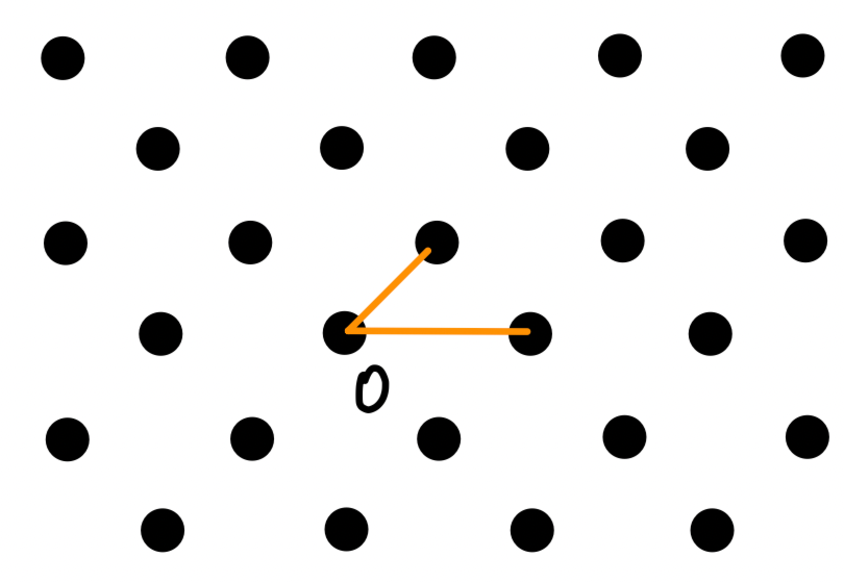
\includegraphics[width=0.45\textwidth]{goodbasis1}%
		\hspace{20pt}
		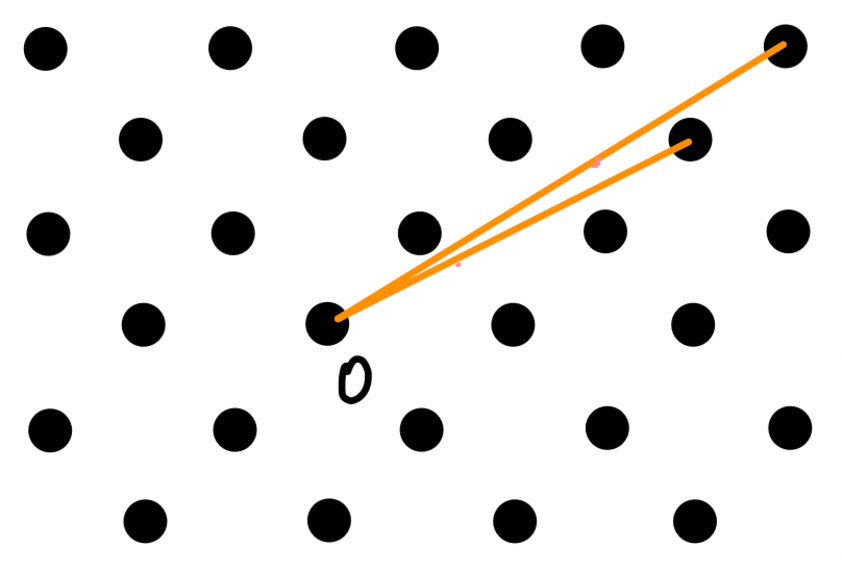
\includegraphics[width=0.45\textwidth]{badbasis1} \\[10pt]
		\Large
		\centering
		Хороший базис \hspace{60pt} Плохой базис

	\end{frame}
}

{
	\setbeamercolor{background canvas}{bg=white}
	\setbeamercolor{title}{fg=black}
	\setbeamercolor{frametitle}{fg=black}
	\setbeamercolor{normal text}{fg=black}\usebeamercolor*{normal text}
	\begin{frame}{Шифрование на решетках II}
		%\pause
		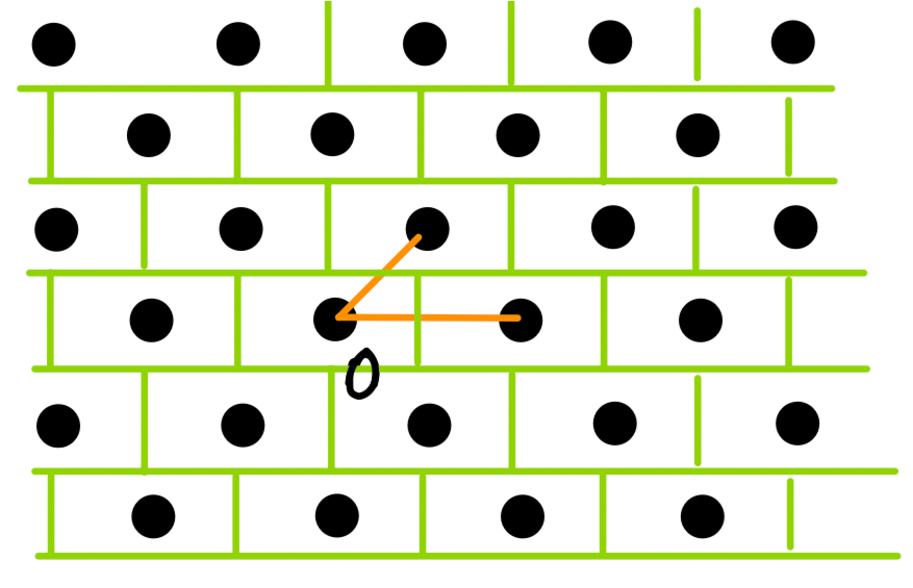
\includegraphics[width=0.45\textwidth]{goodbasis2}%
		\hspace{20pt}
		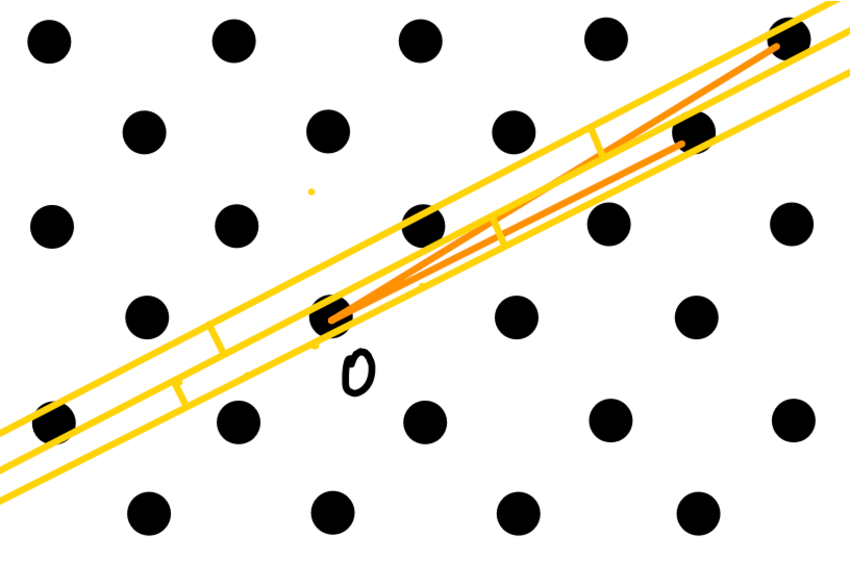
\includegraphics[width=0.45\textwidth]{badbasis2} \\[10pt]
		\Large
		\centering
		Грам-Шмидт базисы
	\end{frame}
}

{
	\setbeamercolor{background canvas}{bg=white}
	\setbeamercolor{title}{fg=black}
	\setbeamercolor{frametitle}{fg=black}
	\setbeamercolor{normal text}{fg=black}\usebeamercolor*{normal text}
	\begin{frame}{Шифрование на решетках III}
		%\pause
		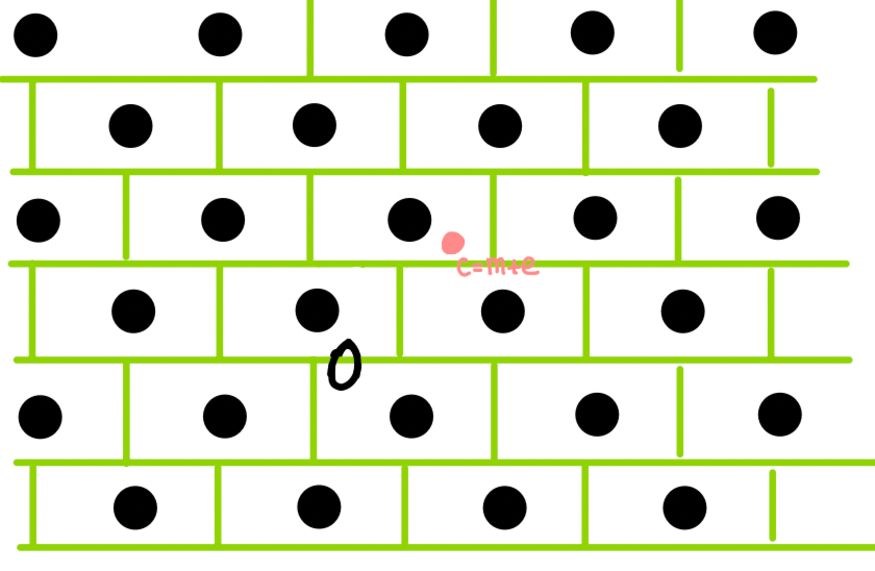
\includegraphics[width=0.45\textwidth]{goodbasis3}%
		\hspace{20pt}
		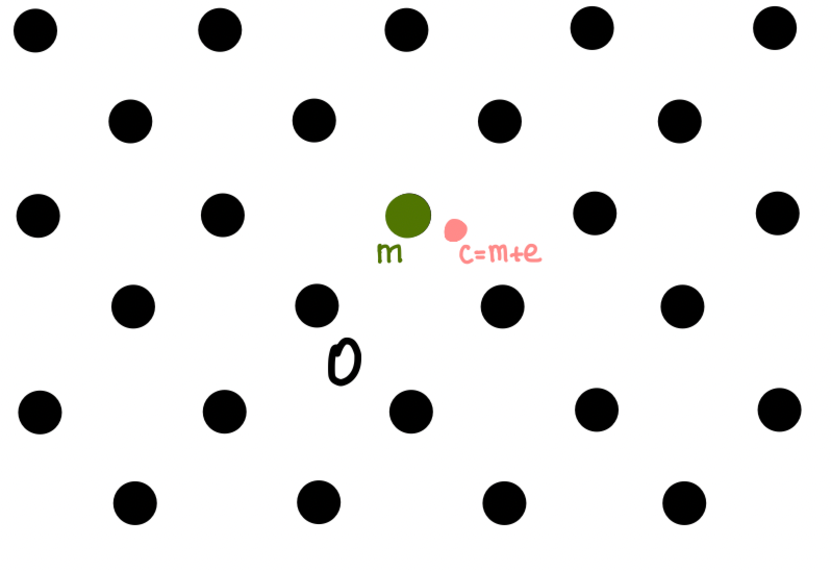
\includegraphics[width=0.45\textwidth]{badbasis3} \\[10pt]
		\Large
		\centering
		Шифрование сообщения $m$
	\end{frame}
}

{
	\setbeamercolor{background canvas}{bg=white}
	\setbeamercolor{title}{fg=black}
	\setbeamercolor{frametitle}{fg=black}
	\setbeamercolor{normal text}{fg=black}\usebeamercolor*{normal text}
	\begin{frame}{Что если использовать разные решетки?}
		%\pause
		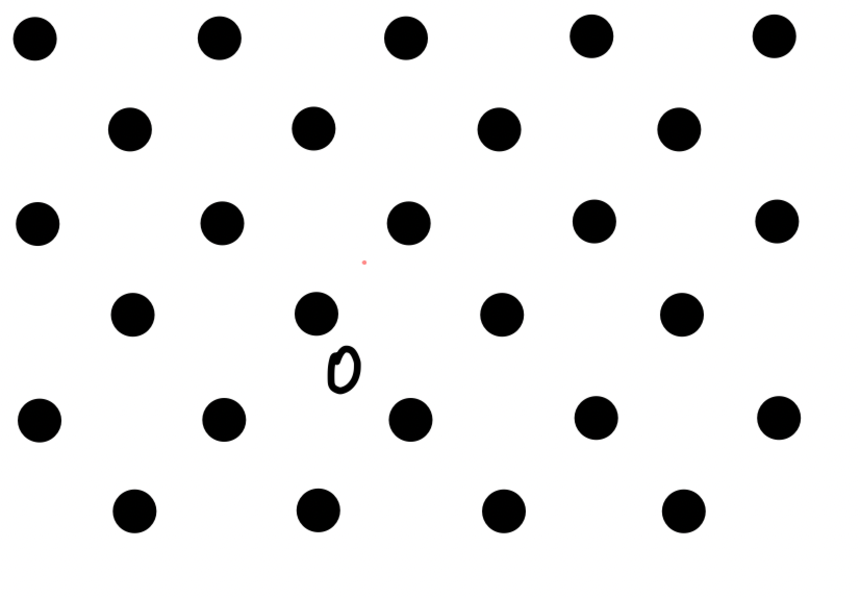
\includegraphics[width=0.45\textwidth]{goodbasis4}%
		\hspace{20pt}
		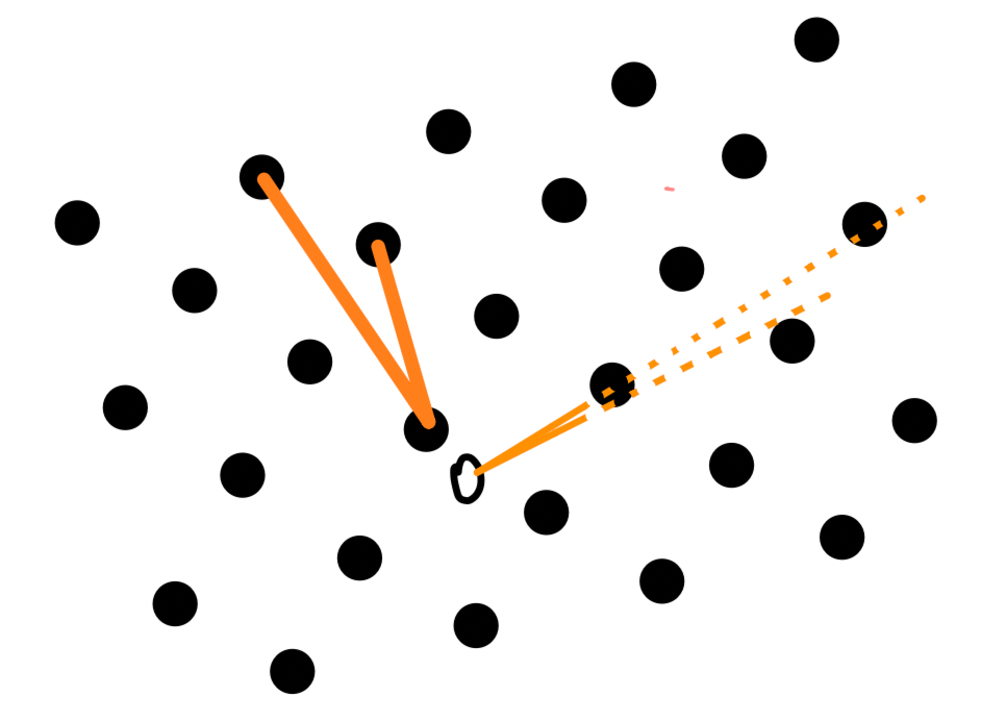
\includegraphics[width=0.45\textwidth]{badbasis4} \\[10pt]
		\Large
		\centering
		$\mathcal{L}$ \hspace{150pt} $O\cdot \mathcal{L}, O \in \mathcal{O}_n(\R)$
		
	\end{frame}
}

{
	\setbeamercolor{background canvas}{bg=white}
	\setbeamercolor{title}{fg=black}
	\setbeamercolor{frametitle}{fg=black}
	\setbeamercolor{normal text}{fg=black}\usebeamercolor*{normal text}
	\setbeamercolor{itemize item}{fg=black}
\begin{frame}{Задача Изоморфизма Решеток (Lattice Isomorphism Problem)}
	\Large 
	
	По заданным базисам $B, B' \in \R^{n\times n}$, найти $O \in \mathcal{O}_n(\R)$ и $U \in \mathtt{GL}_n(\R)$, чтобы выполнялось:
	\[
		B' = O \cdot B \cdot U. 
	\]
	
	\begin{itemize}
		\item $\mathtt{Min}(\Lat(B')) = O \cdot \mathtt{Min}(\Lat(B)) $
		\item На практике решается нахождение коротких векторов в $\mathcal{L}(B)$ и $\mathcal{L}(B')$ и нахождение изометрии между ними
		\item LIP лежит в основе подписи HAWK
	\end{itemize}
	
\end{frame}
}

\begin{frame}{Открытые вопросы}
\large
\begin{enumerate}
	\setlength\itemsep{5pt}
	 
	\item Улучшенные алгоритмы SVP  для алгебраических решёток: алгебраический LLL (для алг.\ нормы), SVP, BKZ
	\item Практический анализ LWE, NTRU
	\item Анализ `дуальной атаки' на LWE, NTRU
	\item Улучшенная реализация просеивания
	\item Эффективные конструкции на решетках: слепая подпись
	\item Построение решеток из кодов: анализ качества решеток (кратчайшего вектора относительно определителя), построенных из различных кодов
	\item Анализ качества решеток как кодов (актуально для квантовых кодов, исправляющих ошибки)
	\item Криптоанализ задачи Lattice Isomorphism Problem (LIP): по двух решеткам $\mathcal{L}, \mathcal{L'} \subset \R^n$, найти ортонормальную матрицу $O$, т.ч.\ $\mathcal{L'} = O \mathcal{L}$. 

\end{enumerate}


\end{frame}

\end{document}
